\documentclass[11pt]{article}
\usepackage{amsfonts,amssymb,amsmath,amsthm,epsfig,euscript,verbatim,graphicx, pdfpages}
\setlength{\textwidth}{6.3in}
\setlength{\textheight}{8.7in}
\setlength{\topmargin}{0pt}
\setlength{\headsep}{0pt}
\setlength{\headheight}{0pt}
\setlength{\oddsidemargin}{0pt}
\setlength{\evensidemargin}{0pt}
\newtheorem{theorem}{Theorem}
\newtheorem{lemma}[theorem]{Lemma}
\newtheorem{corollary}[theorem]{Corollary}
\newtheorem{definition}[theorem]{Definition}
\newtheorem{conjecture}{Conjecture}

\def\mn{\makebox[1.1ex]{\rule[.58ex]{.71ex}{.15ex}}}

\long\def\symbolfootnote[#1]#2{\begingroup
\def\thefootnote{\fnsymbol{footnote}}\footnote[#1]{#2}\endgroup}

% newcommands to be used in math mode

%\newcommand{\coi}[1][\sigma]{\mathrm{coinv}(#1)}
\newcommand{\coib}[1][\sigma]{\mathrm{coinv}_B(#1)}
\newcommand{\com}[1][\sigma]{\mathrm{comaj}(#1)}
\newcommand{\comb}[1][\sigma]{\mathrm{comaj}_B(#1)}
%\DeclareMathOperator{\des}{\mathrm{des}}
%\DeclareMathOperator{\maj}{\mathrm{maj}}
\newcommand{\desb}[1][\sigma]{\mathrm{des}_B(#1)}
%\newcommand{\epq}[1][t(x-y)]{\mathbf{e}_{p,q}^{#1}}
\newcommand{\HF}{\xi}
\newcommand{\HK}{\xi_B}
%\newcommand{\inv}[1]{\mathrm{inv}(#1)}
\newcommand{\invb}[1]{\mathrm{inv}_B(#1)}
\newcommand{\la}{\lambda}
\newcommand{\La}{\Lambda}
\newcommand{\ris}[1]{\mathrm{ris}(#1)}
\newcommand{\wris}[1]{\mathrm{wris}(#1)}
\newcommand{\sris}[1]{\mathrm{sris}(#1)}
\newcommand{\wmaj}[1][\gamma]{\mathrm{wmaj}(#1)}
\newcommand{\wdes}[1]{\mathrm{wdes}(#1)}
\newcommand{\sdes}[1]{\mathrm{sdes}(#1)}
\newcommand{\des}[1]{\mathrm{des}(#1)}
\newcommand{\levmaj}[1][\gamma]{\mathrm{levmaj}(#1)}
\newcommand{\lev}[1][\gamma]{\mathrm{lev}(#1)}
\DeclareMathOperator{\parts}{parts}
\newcommand{\majb}[1][\sigma]{\mathrm{maj}_B(#1)}
\newcommand{\mmaj}[1][\sigma^1,\dots,\sigma^m]{\mathrm{commaj}(#1)}
\newcommand{\mdes}[1][\sigma^1,\dots,\sigma^m]{\mathrm{comdes}(#1)}
\newcommand{\nega}[1][\sigma]{\mathrm{neg}(#1)}
\newcommand{\nth}[1][n]{{#1}^{\mathrm{th}}}
\newcommand{\ov}{\overline}
\newcommand{\pos}[1][\sigma]{\mathrm{pos}(#1)}
\newcommand{\qbinom}[2]{\genfrac{[}{]}{0pt}{}{#1}{#2}_{q}}
\newcommand{\pqbinom}[2]{\genfrac{[}{]}{0pt}{}{#1}{#2}_{p,q}}
\newcommand{\rbinom}[2]{\genfrac{[}{]}{0pt}{}{#1}{#2}_{r}}
%\newcommand{\ris}[1][\sigma]{\mathrm{ris}(#1)}
%\newcommand{\risb}[1][\sigma]{\mathrm{ris}_B(#1)}
\newcommand{\sg}{\sigma}
\newcommand{\ep}{\epsilon}
\newcommand{\ga}{\gamma}
\newcommand{\Ta}{\Theta}
\newcommand{\N}{\mathbb{N}}
\newcommand{\Pos}{\mathbb{P}}
\newcommand{\Ev}{\mathbb{E}}
\newcommand{\Odd}{\mathbb{O}}
\newcommand{\sP}{s\mathbb{P}}
\newcommand{\UD}{U\mbox{-}D}
\newcommand{\NDD}{ND\mbox{-}D}
\newcommand{\UNU}{U\mbox{-}NU}
\newcommand{\ud}{u\mbox{-}d}
\newcommand{\ndd}{nd\mbox{-}d}
\newcommand{\unu}{u\mbox{-}nu}
\def\dd{{\textrm d}}
%\def\qexp{{\mathbf{e}}_q}
%\def\pqexp{{\mathbf{e}}_{p,q}}


\newcommand{\al}{\alpha}
\newcommand{\cref}[1]{Corollary \ref{corollary:#1}}
\newcommand{\cmch}[1][\sg^1,\dots,\sg^m]{\text{$\tau$-$\mathrm{commch}$}(#1)}
\newcommand{\clap}[1][\sg^1,\dots,\sg^m]{\text{$\tau$-$\mathrm{comnlap}$}(#1)}
\newcommand{\cvlap}[1][w,y]{\text{$v$-$\mathrm{comnlap}$}(#1)}
%\newcommand{\des}[1]{\mathrm{des}(#1)}
%\newcommand{\ep}[1]{\exp \left( #1 \right)}
\newcommand{\qexp}[1]{\exp_{q} \left( #1 \right)}
\newcommand{\pqexp}[1]{\exp_{q,p} \left( #1 \right)}
\newcommand{\Epq}[1]{\mathrm{Exp}_{q} \left( #1 \right)}
\newcommand{\eref}[1]{\eqref{equation:#1}}
\newcommand{\FA}{f}
\newcommand{\FAq}{f_q}
\newcommand{\FAm}{f_m}
\newcommand{\FB}{g}
\newcommand{\FBb}{g_2}
%\newcommand{\fig}[1]{\vspace{1ex} \begin{center} \input{#1.pstex_t} \end{center%} \vspace{1ex}}
\newcommand{\Floor}[1][n/2]{\left \lfloor #1 \right \rfloor}
\newcommand{\HA}{\xi}
\newcommand{\HAq}{\xi_q}
\newcommand{\HAm}{\xi_m}
\newcommand{\HB}{\varphi}
\newcommand{\HC}{\eta}
\newcommand{\HCb}{\eta_2}
\newcommand{\HL}{\vartheta}
\newcommand{\im}{i}
\newcommand{\inv}[1]{\mathrm{inv}(#1)}
\newcommand{\coinv}[1]{\mathrm{coinv}(#1)}
%\newcommand{\La}{\Lambda}
%\newcommand{\la}{\lambda}
\newcommand{\lref}[1]{Lemma \ref{lemma:#1}}
%\newcommand{\nth}[1][n]{{#1}^{\mathrm{th}}}
\newcommand{\qbin}[3]{\genfrac{[}{]}{0pt}{}{#1}{#2}_{#3}}
\newcommand{\red}[1]{\mathrm{red}(#1)}
%\newcommand{\sg}{\sigma}
\newcommand{\sm}[2]{\sum_{#1 = #2}^{\infty}}
\newcommand{\sref}[1]{Section \ref{sub:#1}}
\newcommand{\tlap}[1]{\text{$\tau$-$\mathrm{nlap}$}(#1)}
\newcommand{\tmch}[1]{\text{$\tau$-$\mathrm{mch}$}(#1)}
\newcommand{\umch}[1]{\text{$u$-$\mathrm{mch}$}(#1)}
\newcommand{\ulap}[1]{\text{$u$-$\mathrm{nlap}$}(#1)}
\newcommand{\tumch}[1]{\text{$(\tau,u)$-$\mathrm{mch}$}(#1)}
\newcommand{\tulap}[1]{\text{$(\tau,u)$-$\mathrm{nlap}$}(#1)}
\newcommand{\Umch}[1]{\text{$\Upsilon$-$\mathrm{mch}$}(#1)}
\newcommand{\Ulap}[1]{\text{$\Upsilon$-$\mathrm{nlap}$}(#1)}
\newcommand{\tref}[1]{Theorem \ref{theorem:#1}}
\newcommand{\vartmch}[2]{\text{${#1}$-mch}(#2)}
\newcommand{\vlap}[1]{\text{$v$-$\mathrm{nlap}$}(#1)}
\newcommand{\vmch}[1]{\text{$v$-$\mathrm{mch}$}(#1)}
\newcommand{\WE}{\upsilon}


% newcommands to be used in regular mode


\newcommand{\fig}[2]{\begin{figure}[ht]
\centerline{\scalebox{.66}{\epsfig{file=#1.eps}}}
\caption{#2}
\label{figure:#1}
\end{figure}}
%\newcommand{\eref}[1]{(\ref{equation:#1})}
%\newcommand{\sref}[1]{Section \ref{sub:#1}}
%\newcommand{\tref}[1]{Theorem \ref{theorem:#1}}
%\newcommand{\lref}[1]{Lemma \ref{lemma:#1}}
%\newcommand{\fref}[1]{Figure \ref{figure:#1}}
\title{PSM Project Status Report: 2}
\author{
Shane Bari\footnote{Supported by "out of pocket"}\\
\small University of Wisconsin-Stout\\[-0.8ex]
\small \texttt{baris0074@my.uwstout.edu}
\and
Russell Chamberlain\addtocounter{footnote}{0}\footnotemark[\value{footnote}]\\
\small University of Wisconsin-Stout\\[-0.8ex]
\small \texttt{chamberlainr0202.my.uwstout.edu}
\and
Cassie Dale\addtocounter{footnote}{0}\footnotemark[\value{footnote}]\\
\small University of Wisconsin-Stout\\[-0.8ex]
\small \texttt{dalec0190@my.uwstout.edu}
\and
Jared Siverling\addtocounter{footnote}{0}\footnotemark[\value{footnote}]\\
\small University of Wisconsin-Stout\\[-0.8ex]
\small \texttt{siverlingj@uwstout.edu}
\and
Keith Wojciechowski\addtocounter{footnote}{0}\footnotemark[\value{footnote}]\\
\small Department of Mathematics\\[-0.8ex]
\small University of Wisconsin, Stout\\[-0.8ex]
\small \texttt{wojciechowskik@uwstout.edu}
%ls
}

\date{\small Submitted: 10/28/15;  Accepted: 10/28/15;  Published: Date 3.}

\begin{document}
\maketitle

\abstract{The following is a summary of work done from 10/8/15 until 10/29/15 as well as future plans for the project.}


\section*{\hspace{-.5cm}Moving Averages}\label{RA}
There are multiple moving, also called rolling, averages---some are listed later in the Future Plans section. After researching, we have limited our scope to two rolling average types: Exponential Moving Average and Simple Moving Average. Additional rolling averages will be considered in the future and added as a later consideration after preliminary model testing is successful.

\subsection*{Simple Moving Average: SMA}\label{SMA}
Simple rolling average is the rolling average utilizing arithmatic mean.\textsuperscript{\cite{INV}} This average is the easist to undrestand and impliment. The preliminary model was first constructed solely using SMAs.

SMA over an $N$-day period at day $t$:
\[
SMA(t) = \frac{\sum_{n=t-N}^{t}\text{data}[n]}{N}
\]

\subsection*{Exponential Moving Average: EMA}\label{EMA}
Exponential Moving Average (EMA) is similar to SMA, however more weight is given to recent data. EMA reacts faster to large price changes compared to SMA. Typically short-term EMA’s such as 12- and 26-day averages are used to calculate indicator variables (moving average convergence divergence, percentage price oscillator, etc.) while long-term EMA’s are usually 50- to 200-day.\cite{INV}
 
EMA over an $N$-day period at day $t$:
\[
\alpha = \frac{2}{1+N}
\]
\[
EMA(t) = (price(t) * \alpha) + (EMA(t-1) * (1-\alpha))
\]

\section*{\hspace{-.5cm} Preliminary Model}\label{PM}
We currently have separate SMA and EMA constructed models that will be combined after additional testing and siginificance has been determined. We are also looking into adding or substituting other moving averages---see Future Plans section. There is a noticable difference between SMA and EMA. Each average has its own short commings and we have already noticed some of them. EMA, for example, has significantly less lag time than SMA, but this can cause a problem with smaller intervals of EMAs. Since the EMA gives more weight to newer values, it is quicker to react and does so with greater strength. This can lead to the EMA being as chaotic as the data it is supposed to help predict, making it of little value. But, SMA has a its own short commings, as seen by the following graphs on the next pages (red is data, green is the EMA, and light blue is the SMA). The plots show different areas where EMA (gree) is higher and when SMA (blue) is higher. The EMA (green) tends to be between the data (red) and SMA (blue).

This comes to no suprise considering some of the results in \textit{Plotting 'timeSeries' Objects} by Wurtz and Setz when they were considering a graph of an EMA with different data from the fTrading package, page 51.\textsuperscript{\cite{WS}} Considering the three plots below, we can see when EMA has larger gaps between itself and the actual data, and when the EMA hugs the data closely. Noticte, the EMA is closer to the data in the middle graph but has large gaps in the upper and lower graphs.

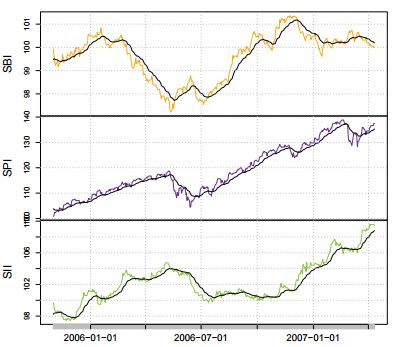
\includegraphics[]{WSEMAplots.jpg}

Notice, SMA can be too 'smooth' and is not senitive enough to follow the data close enough to trigger notifications for buying and selling. We knew this was try from previous readings about large interval rolling averages, but has been seen for smaller interval SMAs. It seems the data's variation and relative 'smoothness' determines which estimator (EMA or SMA) is more useful. It is for this reason, we hope to make a model that detects the variation/amplitude of stocks and uses the appropreate moving average that is more applicable to the situtation.

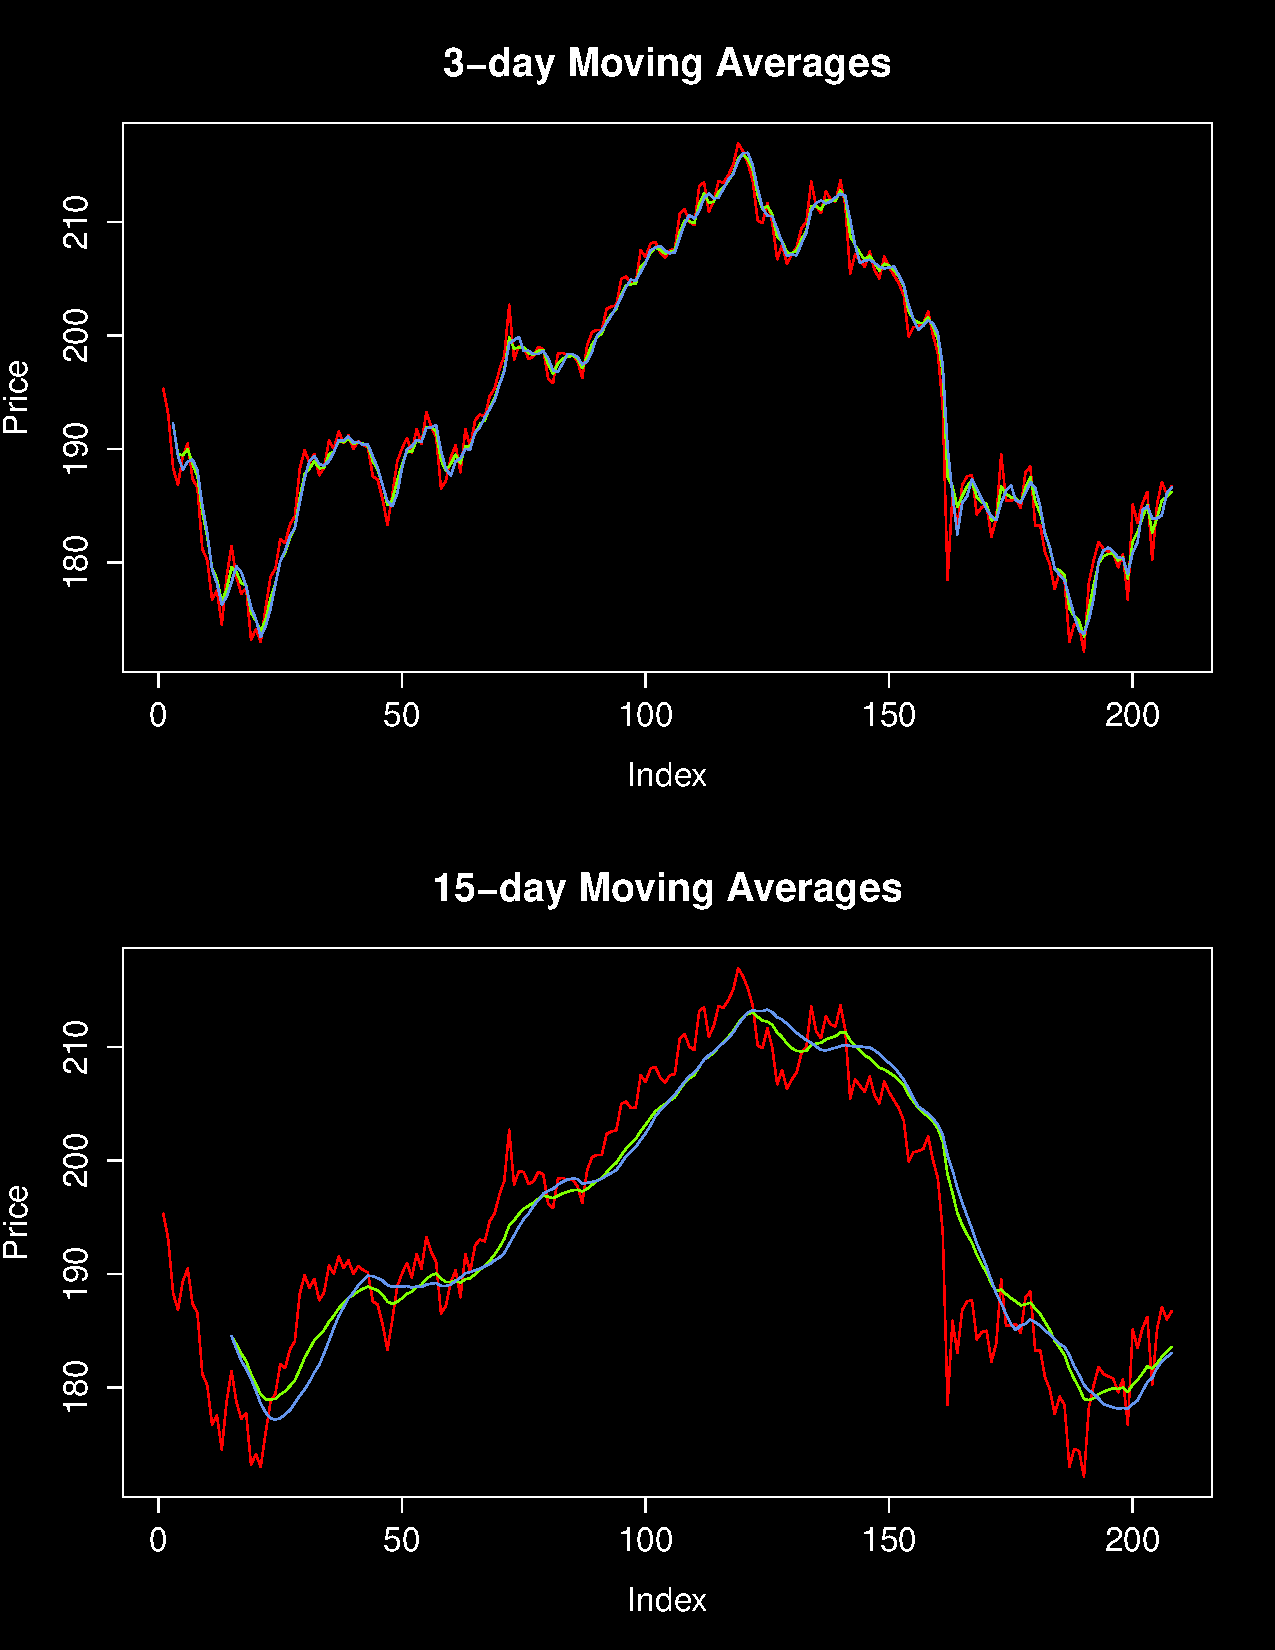
\includepdf{SMAEMAComparisonPlots.pdf}

\subsection*{Graphical Examples of SMA and EMA}\label{GRAPH}
The following are plots from R listing Goldman Stacks Stock information as well as a SMA 3 day and 15 day and an EMA 3 day and 15 day. These plots used the opening stock prices. Notice, as the number of terms considered in the averages increases, the averages 'smooth' out and are slower to adjust---this is called lag time.\textsuperscript{\cite{INV}} We will utilize the stars on the graph to compare the two moving averages. Each star represents a point where the data is more than the respective moving average. It is difficult to see just by direct comparison, but we can flip back and forth between the pages to notice the change in details.

Looking at the difference in stars on each graph, a viewer suspect that the number is drastically different. It turns out there is little difference in the number of stars, points where the data is above the average, but there is a similar count, with stars being at different points on the graph. There are 109 stars in the 3-day SMA and 112 stars in the 10-day SMA plot. There are 108 stars in the 3-day EMA and 113 stars in the 15-day EMA plot.

%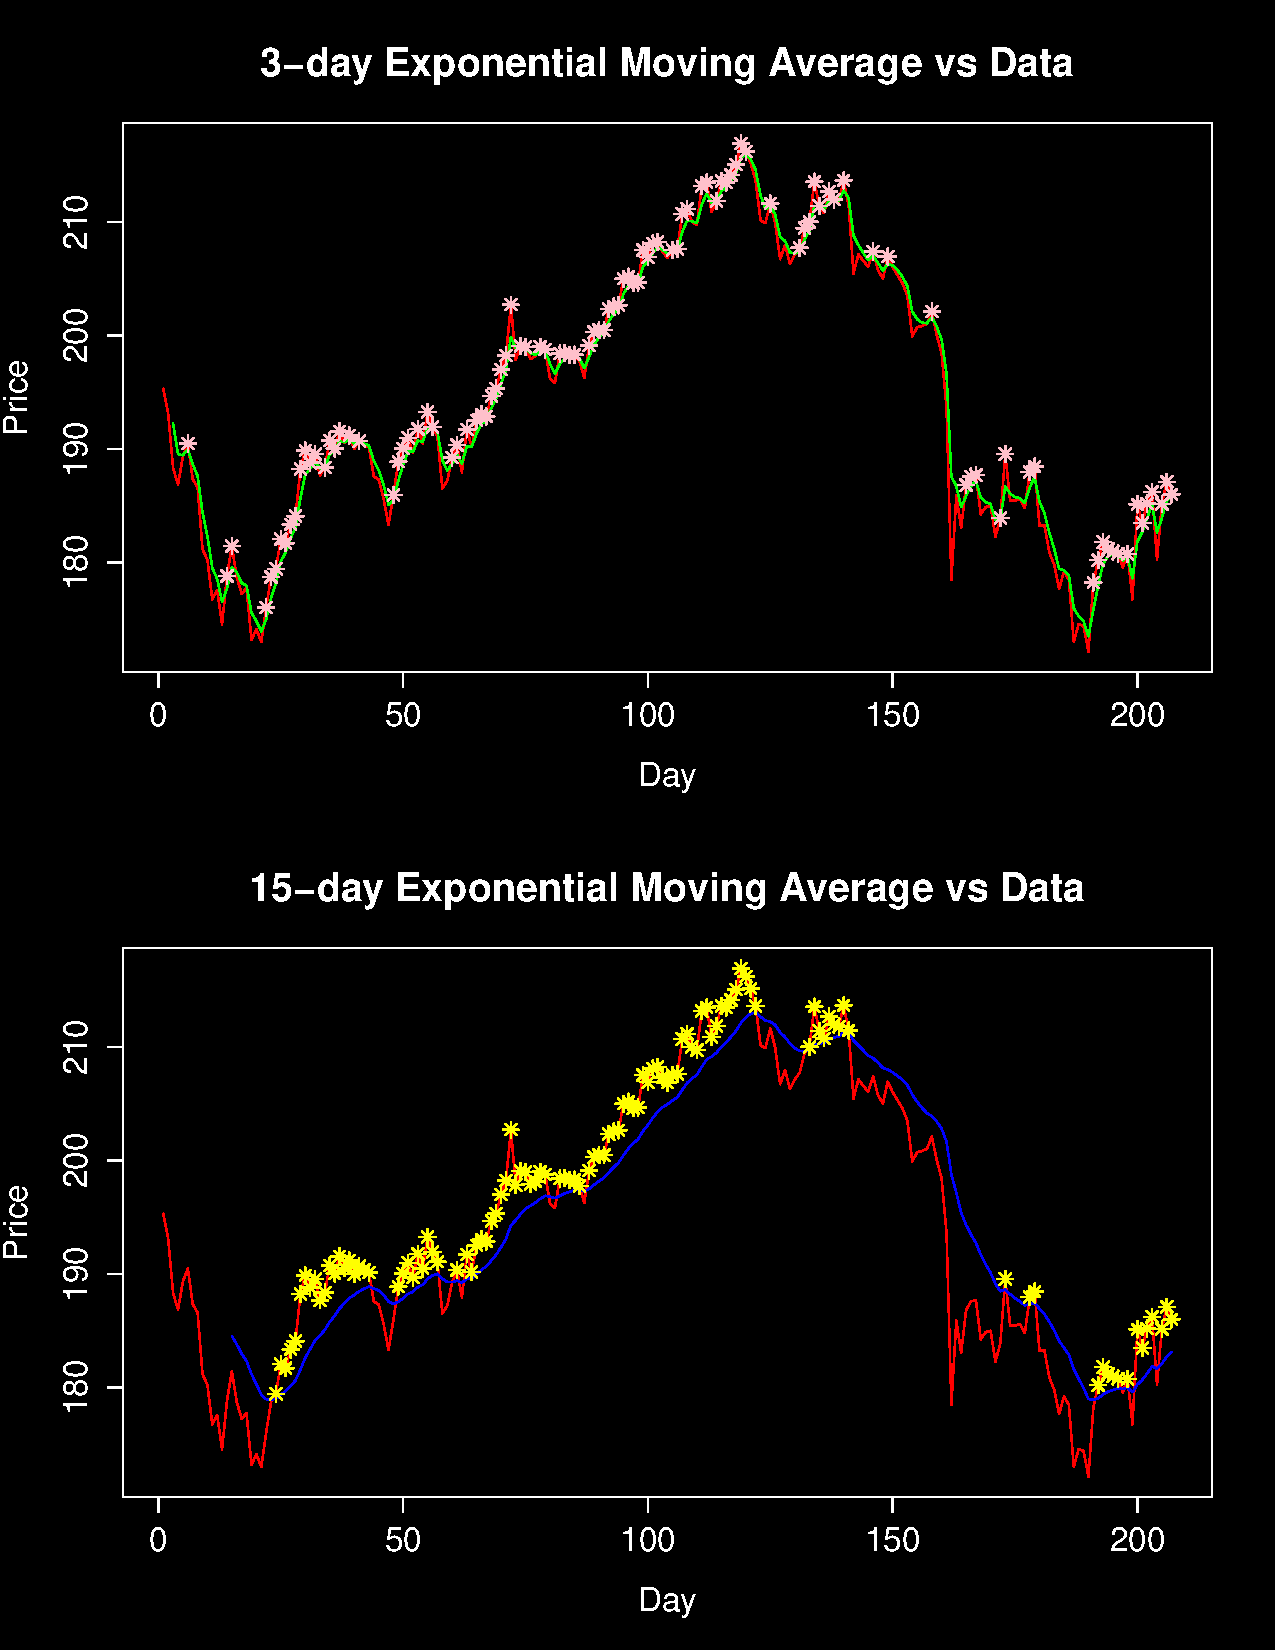
\includegraphics[scale = .5]{EMAplots.pdf}
%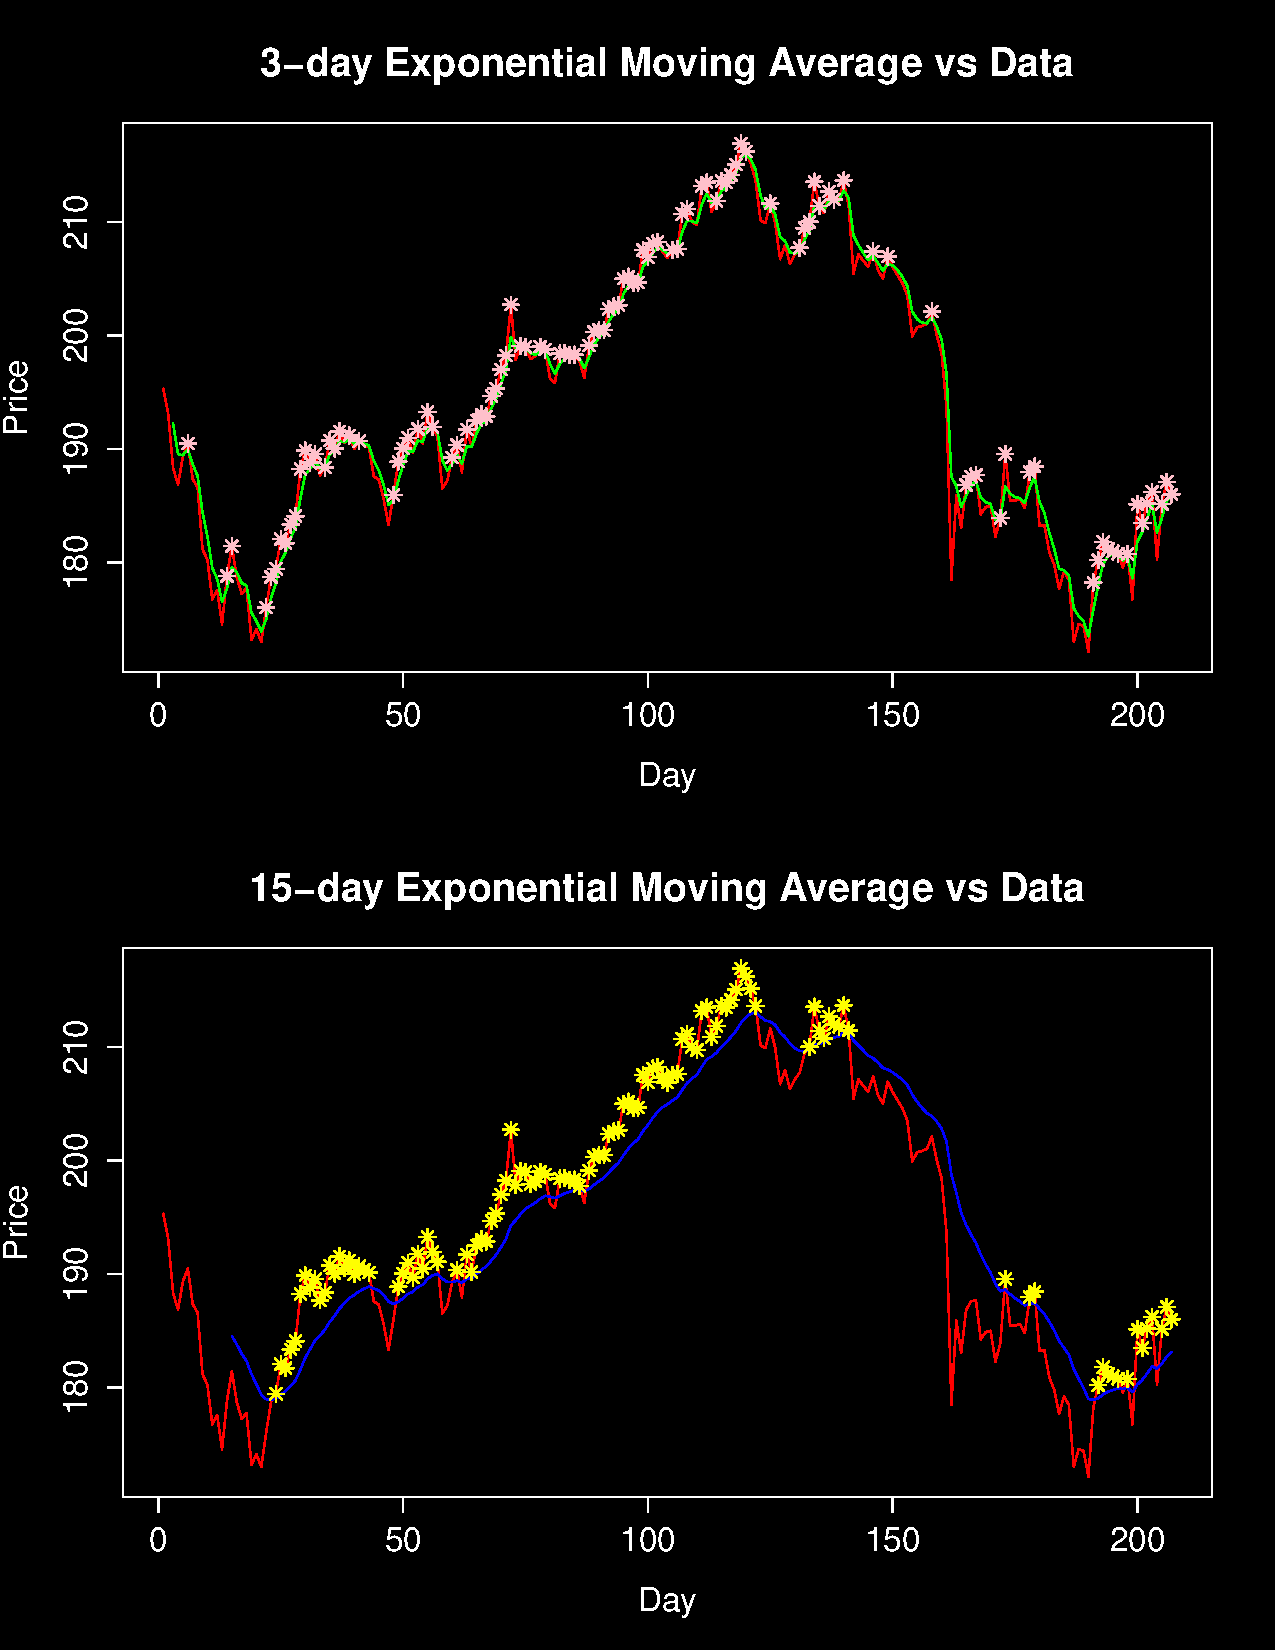
\includepdf[scale=0.8, frame]{EMAplots.pdf}
%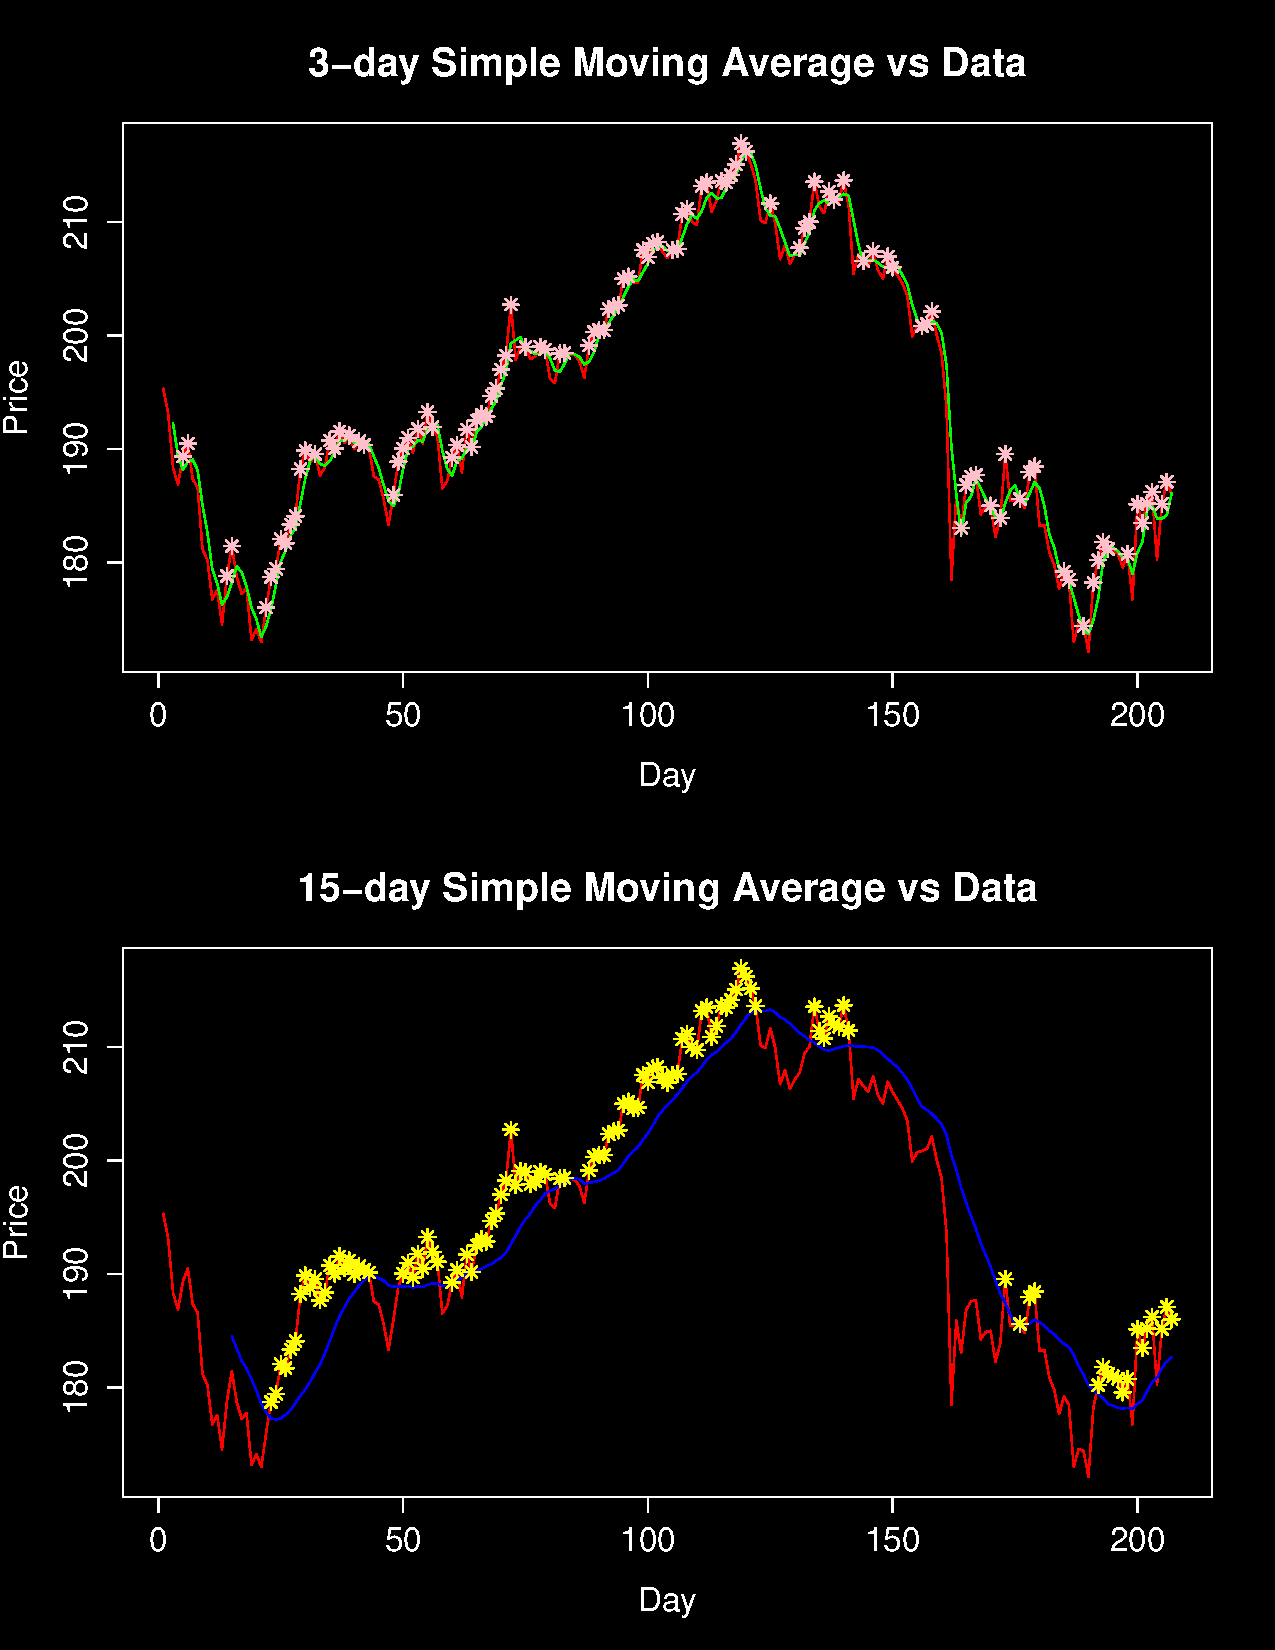
\includepdf[scale=0.8, frame]{SMAplots.pdf}
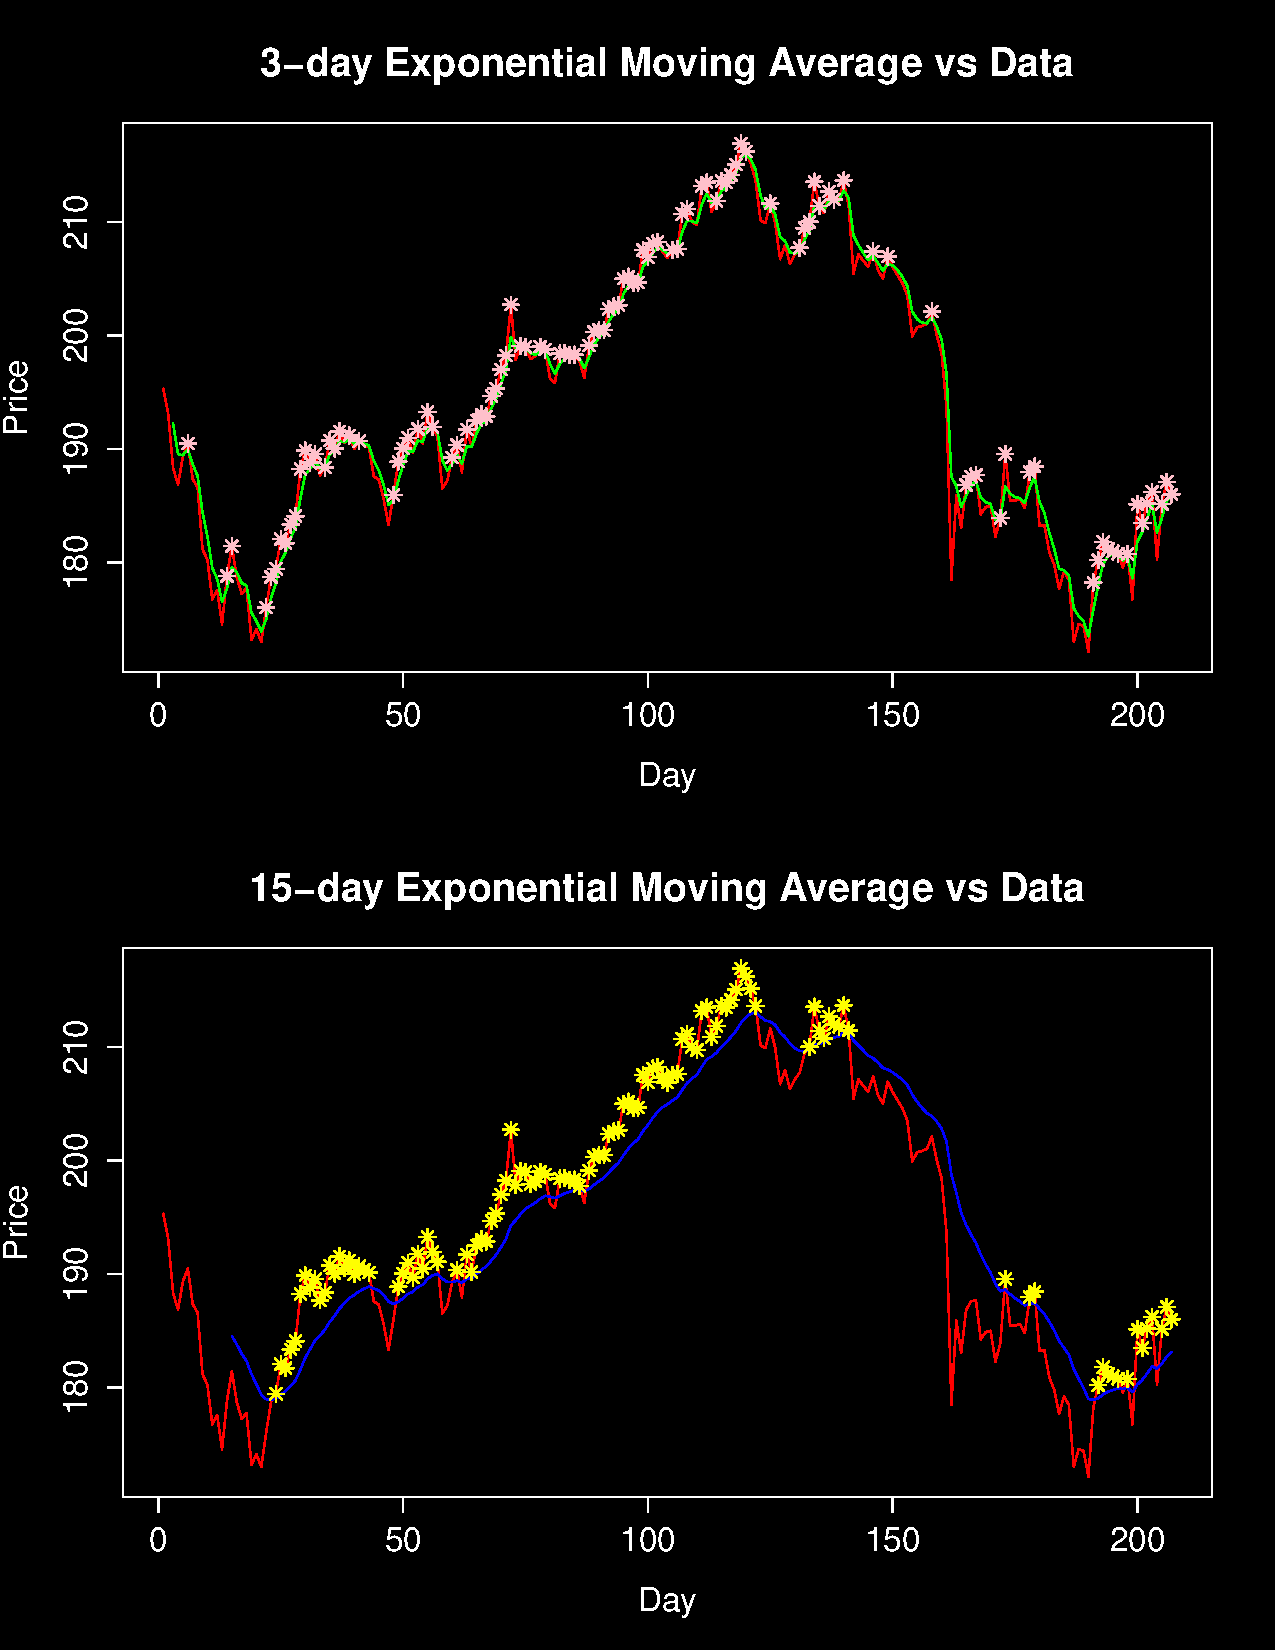
\includepdf[]{EMAplots.pdf}
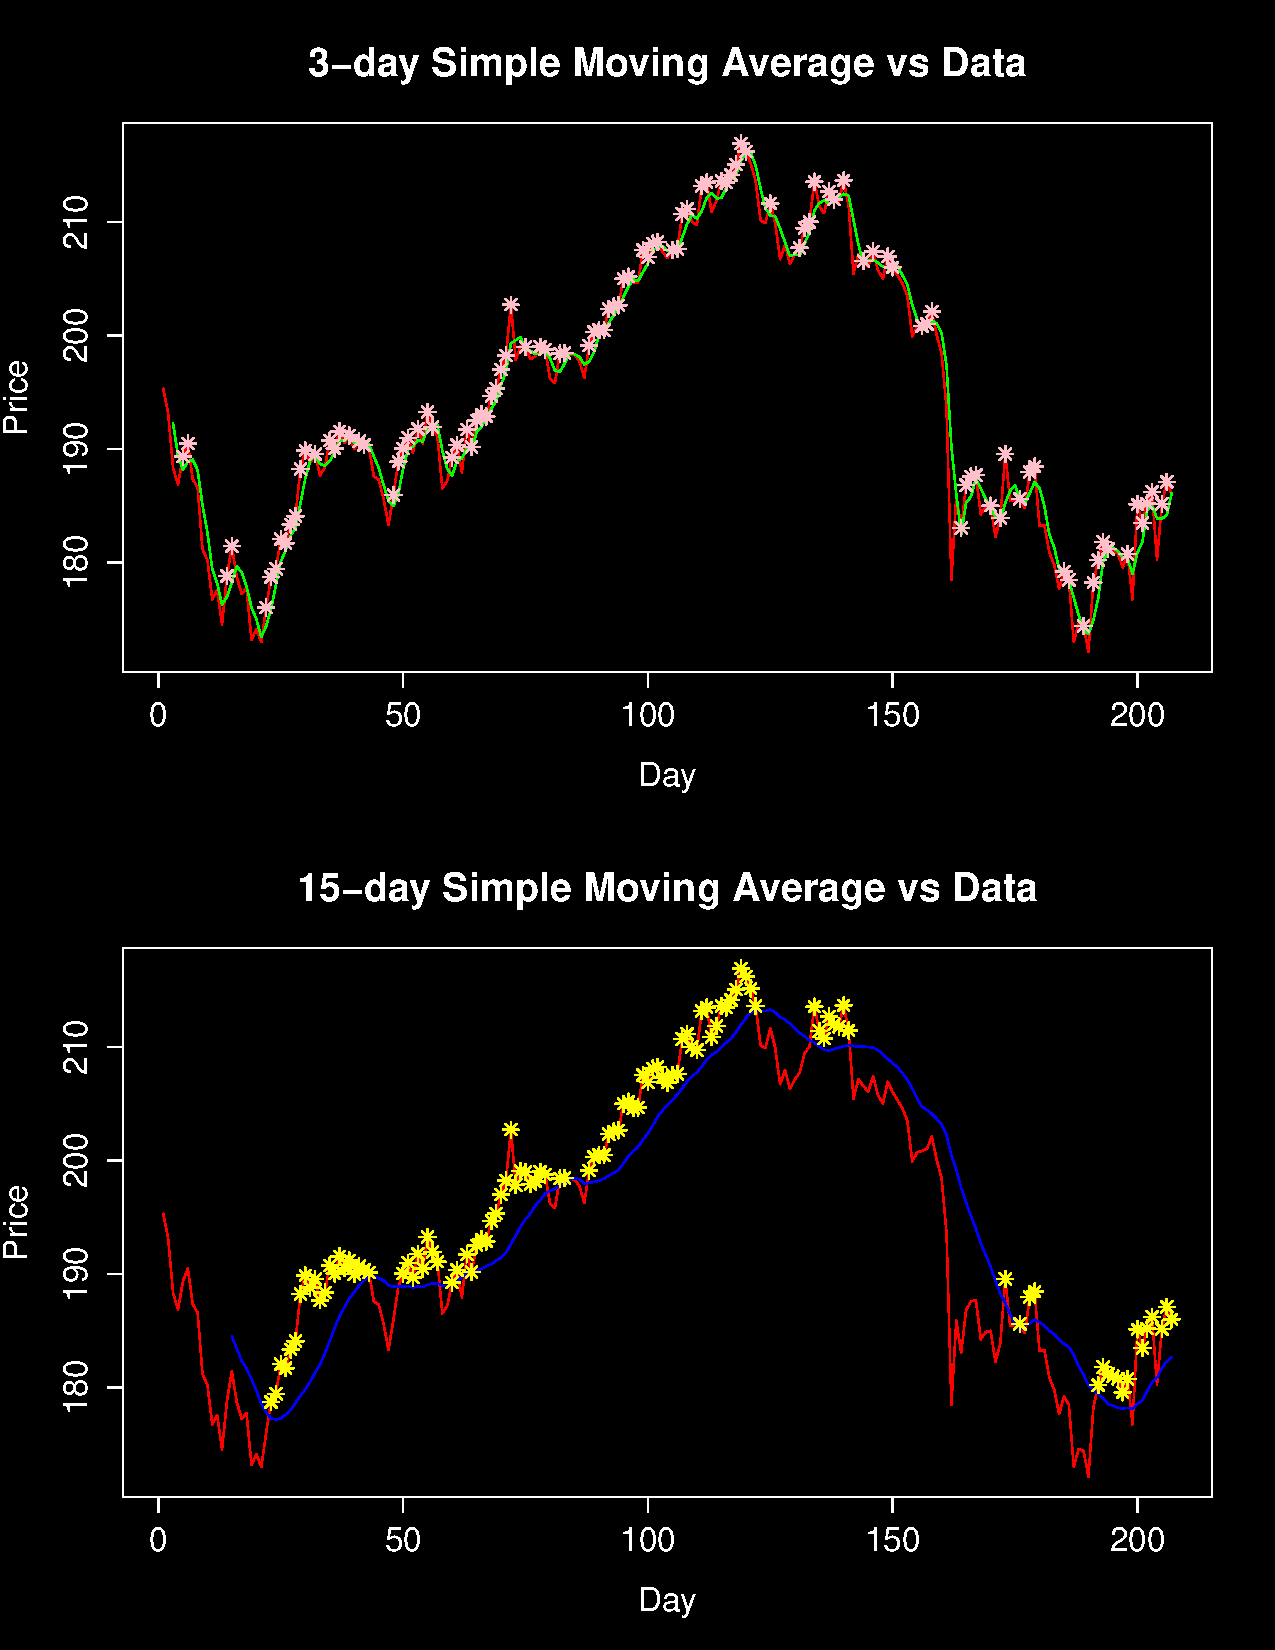
\includepdf[]{SMAplots.pdf}

\section*{\hspace{-.5cm}Future Plans} \label{FP}
This section lists and provides summaries of future topics we are investigating and considering for addition/subsitution into our model.

\subsection*{Choosing Data}
One of the more difficult considerations is what data to use when constructing and testing our model. Do we use opening or closing? Weekly or Daily? Highs or Lows? We are currently researching to help find a superior/significant data to use as a predictor, but most sources seem apathetic and are not willing to argue for one sole data type. We will begin applying different data sets and analyzing.

\subsection*{Golden Cross}
The Golden Cross typically refers to the moment when a 50-day SMA crosses a 200-day SMA. We are considering what intervals of moving averages to use. Is it best to use a smaller interval with a larger interval? Why 50 and 200? What are the benifits and concerns of allowing different day lengths? We will be investigating these further.

\subsection*{Types of Moving Averages}
The following is a non-comprehensive list of different moving averages that can be applied to our model:
\begin{enumerate}
	\item Double Exponential (DEMA)
	\item Triple Exponential (TEMA)
	\item Linear Weighted (LWMA)
	\item Adaptive (AMA)
	\item Hull (HMA)
	\item Jurik (JMA)
\end{enumerate}
We will be investigating applying other moving averages after additional testing with SMA and EMA.

%\subsection*{Horizontal Estimators}
%\This is more of a hypothesis then an actual topic from research. The idea being we can utuilize the intersetion of past horizontal line sigments with current data or moving averages.

\bibliography{MyBiBTeX}
\bibliographystyle{plain}

\end{document}

\begin{thebibliography}{20}

\bibitem{INV} http://www.investopedia.com/terms/s/sma.asp (10/29/2015)

\bibitem{WS} Diethelm Wurtz and Tobias Setz, ETH Zurich and Rmetrics Association Zurich May 12, 2014; https://cran.r-project.org/web/packages/timeSeries/vignettes/timeSeriesPlot.pdf (10/29/15)

\end{thebibliography}


